\documentclass[a4paper,12pt, oneside]{article}
% remplacer "oneside" par "twoside" si on veut imprimer en recto-verso

\usepackage[utf8]{inputenc} % Encodage utf-8
\usepackage[T1]{fontenc} % Nouvelle norme pour codage des caractères
\usepackage{aeguill}

\usepackage[frenchb]{babel} % Règles typographiques françaises, césures
\usepackage{graphicx} % Insertion images
\usepackage{epstopdf} % Converit les images .eps en .pdf pour la compilation avec pdflatex

% package pour tous ce qui est math
\usepackage{amsmath}
\usepackage{amssymb}
\usepackage{amsthm}

% définition de toutes les constantes
\newcommand{\RapportTitre}{Template LaTex}      % Titre

\newcommand{\RapportAuteur}{XXX XXXX} % Auteur 

\newcommand{\RapportDepartement}{XXX}          % Departement
\newcommand{\RapportCours}{XXX}                % le cours

\newcommand{\RapportProfesseur}{XXXXX}   % professeur
\newcommand{\RapportAssistant}{XXXXX}    % assistant

\newcommand{\RapportClasse}{XXXXX}  % la classe
\newcommand{\RapportSalle}{XXX}          % la salle

\newcommand{\RapportDate}{\today}   % la date
\newcommand{\RapportLieu}{XXXXXXX}

% importe les paramètres pour la condifuration du pdf de sortie
\usepackage[colorlinks=true,urlcolor=blue,linkcolor=blue]{hyperref} % créer des hyperliens dans le pdf

% paramètre metadata du pdf
\hypersetup{
    pdftitle={\RapportTitre},%
    pdfauthor={\RapportAuteur},%
    pdfkeywords={rapport} % mot clés
}


% importe tous les paramètres pour afficher du code source
\usepackage{listings} % pour les codes sources
\usepackage{verbatim}
\usepackage{color}
 

\definecolor{gray}{rgb}{0.5,0.5,0.5}
\definecolor{BackColor}{rgb}{0.96,0.96,0.99} %Couleur de fond 
\definecolor{RuleColor}{rgb}{0.9,0.9,0.98} %Couleur de fond 
\definecolor{CmtColor}{rgb}{0.0,0.5,0.0} %Couleur des commentaires
\definecolor{StringColor}{rgb}{0.8,0.0,0.0} %Couleur des chaine de texte
\definecolor{IdentColor}{rgb}{0.0,0.0,0.0} %Couleur des identificateurs
\definecolor{DefColor}{rgb}{0.0,0.0,0.0} %Couleur par defaut (symboles)
\definecolor{WhiteColor}{rgb}{1.0,1.0,1.0} %Couleur par defaut (symboles)    

\lstset{     
    inputencoding=latin1,	 
	 language=C,    % the language of the code
	 basicstyle=\footnotesize \ttfamily,  % the size of the fonts that are used for the code. The type of font is "courrier"
	 numbers=left,   % where to put the line-numbers
	 numberstyle=\tiny\color{gray},  % the style that is used for the line-numbers
	 stepnumber=1,   % the step between two line-numbers. If it's 1, each line 
	    % will be numbered
	 numbersep=5pt,   % how far the line-numbers are from the code
	 backgroundcolor=\color{BackColor},  % choose the background color. You must add \usepackage{color}
	 showspaces=false,   % show spaces adding particular underscores
	 showstringspaces=false,   % underline spaces within strings
	 showtabs=false,   % show tabs within strings adding particular underscores
	 frame=single,    % adds a frame around the code
	 rulecolor=\color{black},   % if not set, the frame-color may be changed on line-breaks within not-black text (e.g. commens (green here))
	 tabsize=2,    % sets default tabsize to 2 spaces
	 captionpos=b,   % sets the caption-position to bottom
	 breaklines=true,    % sets automatic line breaking
	 breakatwhitespace=false,  % sets if automatic breaks should only happen at whitespace
	 %title=\lstname,   % show the filename of files included with \lstinputlisting;
	    % also try caption instead of title
    commentstyle=\color{CmtColor},    %Style des commentaires
    keywordstyle=\color{blue},                %Style des mot clef
    identifierstyle=\color{IdentColor},%Style des identifiant
    stringstyle=\color{StringColor},    %Style des chaines de texte
	 escapeinside={\%*}{*)},  % if you want to add a comment within your code
	 morekeywords={*,...}   % if you want to add more keywords to the set
}
\begin{document}

% change la numérotation des tableaux, figures, listing et equation
\numberwithin{equation}{section}
\numberwithin{figure}{section}
\numberwithin{table}{section}
\numberwithin{lstlisting}{section}


\begin{center}
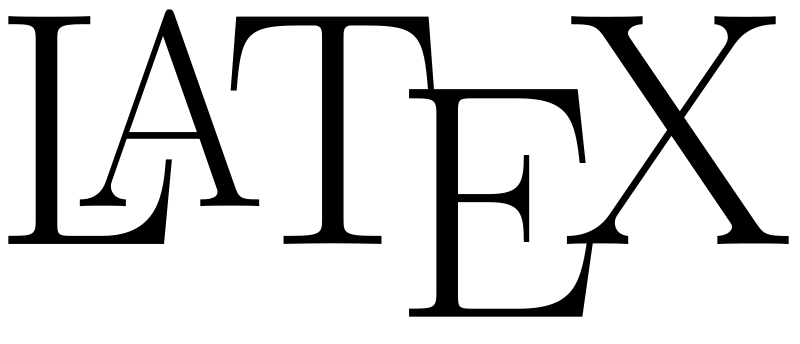
\includegraphics[width=0.3\textwidth]{images/logo.png}\hfill
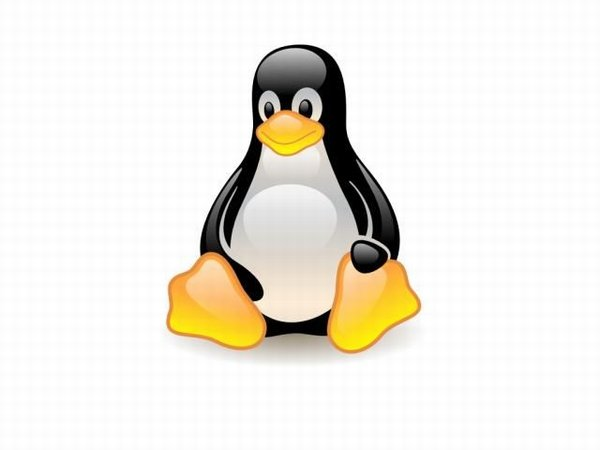
\includegraphics[width=0.4\textwidth]{images/tux.jpg}
\end{center}

\vspace{3cm}


\noindent \hrulefill
\begin{center}
%titre en gras
\huge \RapportTitre
\end{center}
\noindent \hrulefill

\vspace{1cm}
%centrer le tableau
\begin{center}
%tableau sans ligne pour aligner le texte
\begin{tabular}{l l}
Département:          & \RapportDepartement \\
Unité d'enseignement: & \RapportCours \\
\end{tabular}
\end{center}

\vspace{2cm}
 %tableau a gauche
\begin{flushleft}
%tableau sans ligne pour aligner le texte
\begin{tabular}{l l}
Auteur:        & \RapportAuteur \\
\\
Professeur:    & \RapportProfesseur \\
Assistant:     & \RapportAssistant \\
\\
Classe:        & \RapportClasse \\
Salle du labo: & \RapportSalle \\
\\
Date:          & \RapportDate \\
\end{tabular}
\end{flushleft}

\newpage

\tableofcontents

\newpage

\section{Introduction}


\section{Section}

\subsection{sous section}

Dans l'équation \ref{equation de x}.
\begin{equation}
x(t) = \frac{sin(\omega_y \cdot t + \phi)} {t}
\label{equation de x}
\end{equation}


\section{Section 2}

\subsection{sous section 2}



\newpage

\section{Conclusion}


\vspace{5cm}
\RapportLieu, \RapportDate \\

Signature:\\

\RapportAuteur

\newpage

\section{Annexes}

\subsection{code source filtrage.m}
\lstinputlisting[language = matlab]{code_source/filtrage.m}
\label{matlab_filtrage}
\newpage
\end{document}